\documentclass[crop, tikz]{standalone}
\usepackage{tikz}

\usetikzlibrary{positioning}

\tikzstyle{inputNode}=[draw,circle,minimum size=10pt,inner sep=0pt]
\tikzstyle{stateTransition}=[-stealth, thick]

\begin{document}
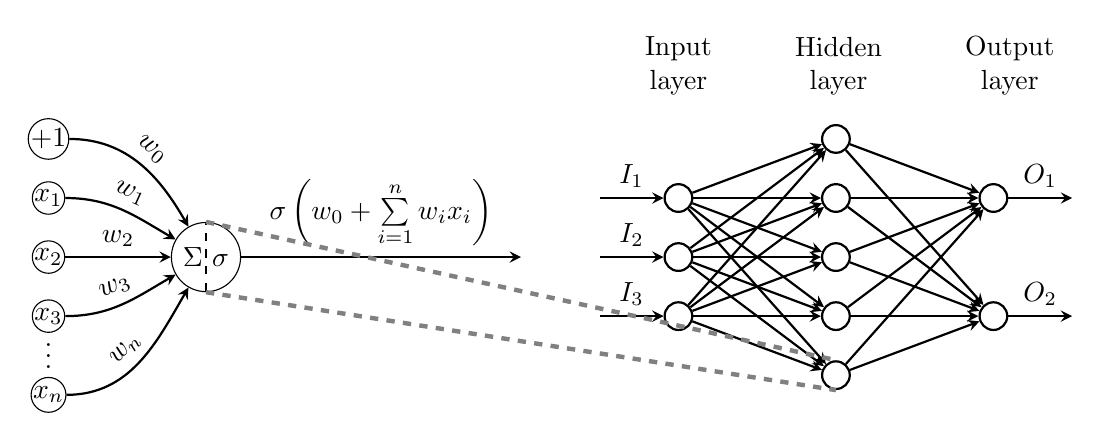
\begin{tikzpicture}
	\node[draw,circle,minimum size=25pt,inner sep=0pt] (x) at (0,0) {$\Sigma$ $\sigma$};

	\node[inputNode] (x0) at (-2, 1.5) {$\tiny +1$};
	\node[inputNode] (x1) at (-2, 0.75) {$\tiny x_1$};
	\node[inputNode] (x2) at (-2, 0) {$\tiny x_2$};
	\node[inputNode] (x3) at (-2, -0.75) {$\tiny x_3$};
	\node[inputNode] (xn) at (-2, -1.75) {$\tiny x_n$};

	\draw[stateTransition] (x0) to[out=0,in=120] node [midway, sloped, above] {$w_0$} (x);
	\draw[stateTransition] (x1) to[out=0,in=150] node [midway, sloped, above] {$w_1$} (x);
	\draw[stateTransition] (x2) to[out=0,in=180] node [midway, sloped, above] {$w_2$} (x);
	\draw[stateTransition] (x3) to[out=0,in=210] node [midway, sloped, above] {$w_3$} (x);
	\draw[stateTransition] (xn) to[out=0,in=240] node [midway, sloped, above] {$w_n$} (x);
	\draw[stateTransition] (x) -- (4,0) node [midway,above] {$\sigma\left(w_0 + \sum\limits_{i=1}^{n}{w_ix_i}\right)$};
	\draw[dashed] (0,-0.43) -- (0,0.43);
	\node (dots) at (-2, -1.15) {$\vdots$};
	\node[inputNode, thick] (i1) at (6, 0.75) {};
	\node[inputNode, thick] (i2) at (6, 0) {};
	\node[inputNode, thick] (i3) at (6, -0.75) {};
	
	\node[inputNode, thick] (h1) at (8, 1.5) {};
	\node[inputNode, thick] (h2) at (8, 0.75) {};
	\node[inputNode, thick] (h3) at (8, 0) {};
	\node[inputNode, thick] (h4) at (8, -0.75) {};
	\node[inputNode, thick] (h5) at (8, -1.5) {};
	
	\node[inputNode, thick] (o1) at (10, 0.75) {};
	\node[inputNode, thick] (o2) at (10, -0.75) {};
	
	\draw[stateTransition] (5, 0.75) -- node[above] {$I_1$} (i1);
	\draw[stateTransition] (5, 0) -- node[above] {$I_2$} (i2);
	\draw[stateTransition] (5, -0.75) -- node[above] {$I_3$} (i3);
	
	\draw[stateTransition] (i1) -- (h1);
	\draw[stateTransition] (i1) -- (h2);
	\draw[stateTransition] (i1) -- (h3);
	\draw[stateTransition] (i1) -- (h4);
	\draw[stateTransition] (i1) -- (h5);
	\draw[stateTransition] (i2) -- (h1);
	\draw[stateTransition] (i2) -- (h2);
	\draw[stateTransition] (i2) -- (h3);
	\draw[stateTransition] (i2) -- (h4);
	\draw[stateTransition] (i2) -- (h5);
	\draw[stateTransition] (i3) -- (h1);
	\draw[stateTransition] (i3) -- (h2);
	\draw[stateTransition] (i3) -- (h3);
	\draw[stateTransition] (i3) -- (h4);
	\draw[stateTransition] (i3) -- (h5);
	
	\draw[stateTransition] (h1) -- (o1);
	\draw[stateTransition] (h1) -- (o2);
	\draw[stateTransition] (h2) -- (o1);
	\draw[stateTransition] (h2) -- (o2);
	\draw[stateTransition] (h3) -- (o1);
	\draw[stateTransition] (h3) -- (o2);
	\draw[stateTransition] (h4) -- (o1);
	\draw[stateTransition] (h4) -- (o2);
	\draw[stateTransition] (h5) -- (o1);
	\draw[stateTransition] (h5) -- (o2);
	
	\node[above=of i1, align=center] (l1) {Input \\ layer};
	\node[right=2.3em of l1, align=center] (l2) {Hidden \\ layer};
	\node[right=2.3em of l2, align=center] (l3) {Output \\ layer};
	
	\draw[stateTransition] (o1) -- node[above] {$O_1$} (11, 0.75);
	\draw[stateTransition] (o2) -- node[above] {$O_2$} (11, -0.75);
	
	\path[dashed, double, ultra thick, gray] (x.north) edge[bend left=0] (h5.north);
	\path[dashed, double, ultra thick, gray] (x.south) edge[bend right=0] (h5.south);
\end{tikzpicture}
\end{document}